\documentclass[12pt]{report}
\usepackage[utf8]{inputenc}
\usepackage[russian]{babel}
%\usepackage[14pt]{extsizes}
\usepackage{listings}
\usepackage{graphicx}
\usepackage{amsmath,amsfonts,amssymb,amsthm,mathtools} 
\usepackage{pgfplots}
\usepackage{filecontents}
\usepackage{float}
\usepackage{comment}
\usepackage{indentfirst}
\usepackage{eucal}
\usepackage{enumitem}
%s\documentclass[openany]{book}
\frenchspacing

\usepackage{indentfirst} % Красная строка

\usetikzlibrary{datavisualization}
\usetikzlibrary{datavisualization.formats.functions}

\usepackage{amsmath}


% Для листинга кода:
\lstset{ %
	language=c,                 % выбор языка для подсветки (здесь это С)
	basicstyle=\small\sffamily, % размер и начертание шрифта для подсветки кода
	numbers=left,               % где поставить нумерацию строк (слева\справа)
	numberstyle=\tiny,           % размер шрифта для номеров строк
	stepnumber=1,                   % размер шага между двумя номерами строк
	numbersep=5pt,                % как далеко отстоят номера строк от подсвечиваемого кода
	showspaces=false,            % показывать или нет пробелы специальными отступами
	showstringspaces=false,      % показывать или нет пробелы в строках
	showtabs=false,             % показывать или нет табуляцию в строках
	frame=single,              % рисовать рамку вокруг кода
	tabsize=2,                 % размер табуляции по умолчанию равен 2 пробелам
	captionpos=t,              % позиция заголовка вверху [t] или внизу [b] 
	breaklines=true,           % автоматически переносить строки (да\нет)
	breakatwhitespace=false, % переносить строки только если есть пробел
	escapeinside={\#*}{*)}   % если нужно добавить комментарии в коде
}


\usepackage[left=2cm,right=2cm, top=2cm,bottom=2cm,bindingoffset=0cm]{geometry}
% Для измененных титулов глав:
\usepackage{titlesec, blindtext, color} % подключаем нужные пакеты
\definecolor{gray75}{gray}{0.75} % определяем цвет
\newcommand{\hsp}{\hspace{20pt}} % длина линии в 20pt
% titleformat определяет стиль
\titleformat{\chapter}[hang]{\Huge\bfseries}{\thechapter\hsp\textcolor{gray75}{|}\hsp}{0pt}{\Huge\bfseries}


% plot
\usepackage{pgfplots}
\usepackage{filecontents}
\usetikzlibrary{datavisualization}
\usetikzlibrary{datavisualization.formats.functions}

\begin{document}
	%\def\chaptername{} % убирает "Глава"
	\thispagestyle{empty}
	\begin{titlepage}
		\noindent \begin{minipage}{0.15\textwidth}
			
\includegraphics[width=\linewidth]{img/b_logo}
		\end{minipage}
		\noindent\begin{minipage}{0.9\textwidth}\centering
			\textbf{Министерство науки и высшего образования Российской Федерации}\\
			\textbf{Федеральное государственное бюджетное образовательное учреждение высшего образования}\\
			\textbf{~~~«Московский государственный технический университет имени Н.Э.~Баумана}\\
			\textbf{(национальный исследовательский университет)»}\\
			\textbf{(МГТУ им. Н.Э.~Баумана)}
		\end{minipage}
		
		\noindent\rule{18cm}{3pt}
		\newline\newline
		\noindent ФАКУЛЬТЕТ $\underline{\text{«Информатика и системы управления»}}$ \newline\newline
		\noindent КАФЕДРА $\underline{\text{«Программное обеспечение ЭВМ и информационные технологии»}}$\newline\newline\newline\newline\newline
		
		\begin{center}
			\noindent\begin{minipage}{1.1\textwidth}\centering
				\Large\textbf{  Отчет по лабораторной работе №6}\newline
				\textbf{по дисциплине <<Компьютерные сети>>}\newline\newline\newline
			\end{minipage}
		\end{center}
		
		\noindent\textbf{Тема} $\underline{\text{Разбиение сети на подсети. Настройка DHCP-сервера в сетевом эмуляторе}}$\newline\newline
		\noindent\textbf{Студент} $\underline{\text{Романов А.В.~~~~~~~~~~~}}$\newline\newline
		\noindent\textbf{Группа} $\underline{\text{ИУ7-73Б~~~~~~~~~~~~~~~~~~~}}$\newline\newline
		\noindent\textbf{Преподаватель} $\underline{\text{Рогозин Н. О.}}$\newline\newline\newline
		
		\begin{center}
			\vfill
			Москва~---~\the\year
			~г.
		\end{center}
	\end{titlepage}


\section*{Задание}

\textbf{Вариант №12.}\\

Для локальной общей сети был выделен частный адрес \textbf{192.168.x.0/24}\\

\textbf{1. Необходимо разделить сеть на 5 подсетей:}

\begin{itemize}
	\item подсети 1 и 5 должны поддерживать до x + 10 устройств;
	\item подсети 2 и 4 должны поддерживать до 5 устройств;
	\item подсеть 3 должна поддерживать только 2 устройства.
\end{itemize}

где x - номер по списку в ЭУ. Использовать не более трёх подсетей с возможностью размещения x + 10 хостов.\\

\textbf{2. Настроить DHCP-сервера для выдачи адресов}

\begin{itemize}
	\item для подсети 1 настроить отдельный DHCP сервер;
	\item для подсети 2 настроить в качестве DHCP сервера маршрутизатор 1;
	\item для подсетей 4 и 5 настроить в качестве DHCP сервера маршрутизатор 2.
\end{itemize}

\section*{Результаты работы}

\subsection*{Разделение IP-адресов на подсети}

В таблице 1 представлено разделение IP-адресов на подсети.

\begin{table}[H]
	\centering
	\label{tab:networks}
	\begin{tabular}{|p{0.8cm}|p{1cm}|p{3cm}|p{3cm}|p{3cm}|p{3.2cm}|}
		\hline
		Но-мер под-се-ти & Ко-ли-чест-во хос-тов & ip подсети & Диапазон адресов & Широкове-щательный адрес & Маска под-сети \\
		\hline
		1 & 30 & 192.168.12.0 & 192.168.12.1-192.168.12.30 & 192.168.12.31 & 255.255.255.224 (/27) \\
		\hline
		2 & 6 & 192.168.12.64 & 192.168.12.65-192.168.12.70 & 192.168.12.71 & 255.255.255.248 (/29) \\
		\hline
		3 & 2 & 192.168.12.80 & 192.168.12.81-192.168.12.82 & 192.168.12.83 & 255.255.255.252 (/30) \\
		\hline
		4 & 6 & 192.168.12.72 & 192.168.12.73-192.168.12.78 & 192.168.12.79 & 255.255.255.248 (/29) \\
		\hline
		5 & 30 & 192.168.12.32 & 192.168.12.33-192.168.12.62 & 192.168.12.63 & 255.255.255.224 (/27) \\
		\hline
	\end{tabular}
	\caption{Разделение на подсети}
\end{table}

\section*{Рабочая схема}

\begin{figure}[H]
	\begin{center}
		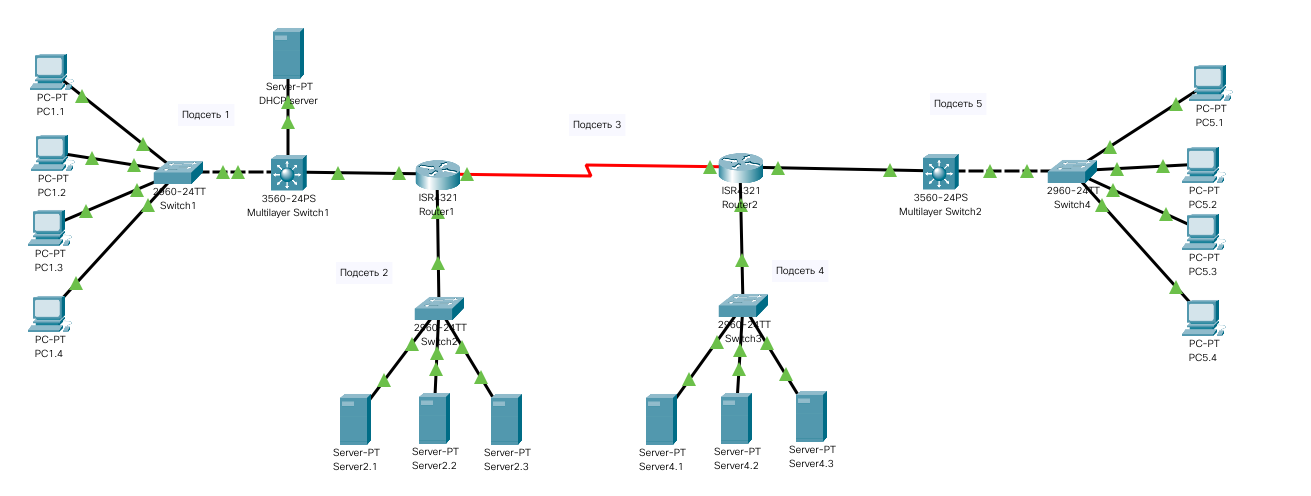
\includegraphics[scale=0.42]{img/1.png}
	\end{center}
	\caption{Схема с настроенными подсетями}
	\label{fig:1}
\end{figure}

\subsection*{Настройка DHCP сервера для 1-ой подсети}

\begin{figure}[H]
	\begin{center}
		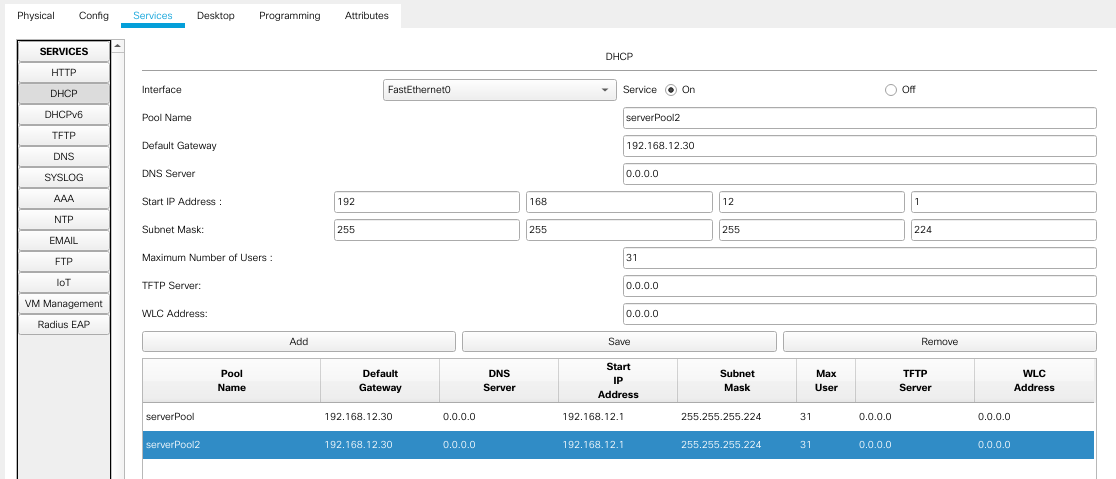
\includegraphics[scale=0.4]{img/2.png}
	\end{center}
	\caption{Настройка сервера}
	\label{fig:2}
\end{figure}

IP-адреса конечным узлам в подсети выдаются автоматически из диапазона сетей подсети №1 (рис. 3). 

\begin{figure}[H]
	\begin{center}
		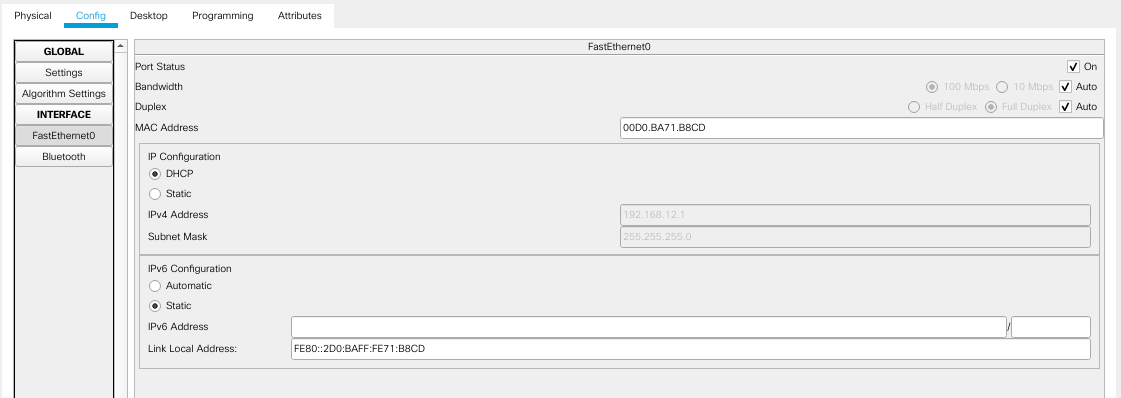
\includegraphics[scale=0.4]{img/3.png}
	\end{center}
	\caption{Автоматически выданный IP-адрес в первой подсети}
	\label{fig:3}
\end{figure}

\begin{figure}[H]
	\begin{center}
		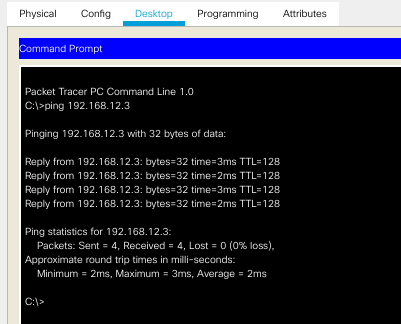
\includegraphics[scale=0.75]{img/4.png}
	\end{center}
	\caption{Проверка связи компьютеров в подсети №1}
	\label{fig:4}
\end{figure}

\subsection*{Настройка DHCP сервера для 2-ой подсети}

\begin{figure}[H]
	\begin{center}
		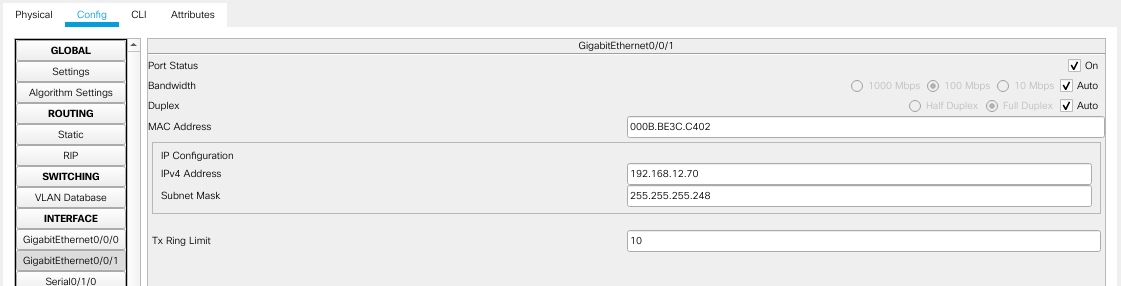
\includegraphics[scale=0.4]{img/5.png}
	\end{center}
	\caption{Настройка муршрутизатора в роли DHCP сервера для подсети №2}
	\label{fig:5}
\end{figure}

\begin{figure}[H]
	\begin{center}
		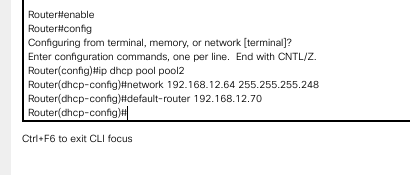
\includegraphics[scale=0.75]{img/6.png}
	\end{center}
	\caption{Настройка маршрутизатора}
	\label{fig:6}
\end{figure}

IP-адреса конечным узлам в подсети выдаются автоматически из диапазона сетей подсети №2 (рис. 7).

\begin{figure}[H]
	\begin{center}
		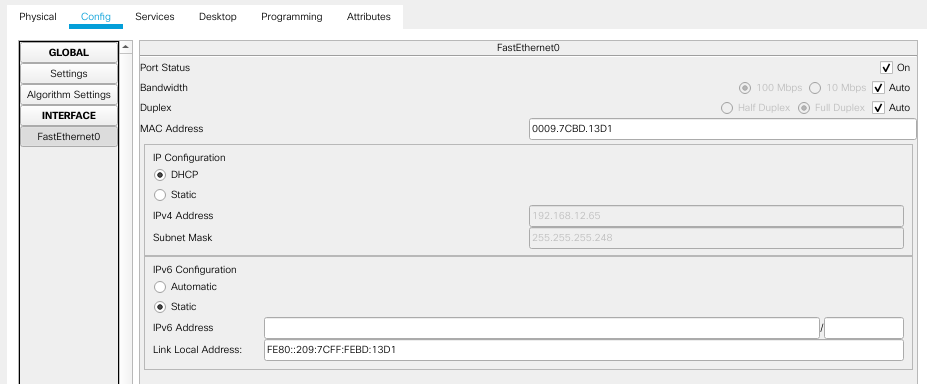
\includegraphics[scale=0.45]{img/7.png}
	\end{center}
	\caption{Автоматически выданный IP-адрес во второй подсети}
	\label{fig:7}
\end{figure}

\begin{figure}[H]
	\begin{center}
		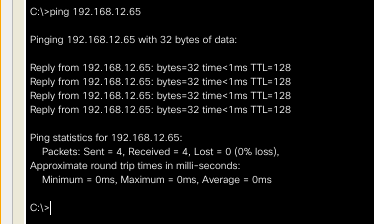
\includegraphics[scale=0.75]{img/8.png}
	\end{center}
	\caption{Проверка связи компьютеров в подсети №2}
	\label{fig:8}
\end{figure}

\subsection*{Настройка 3-ей подсети}

\begin{figure}[H]
	\begin{center}
		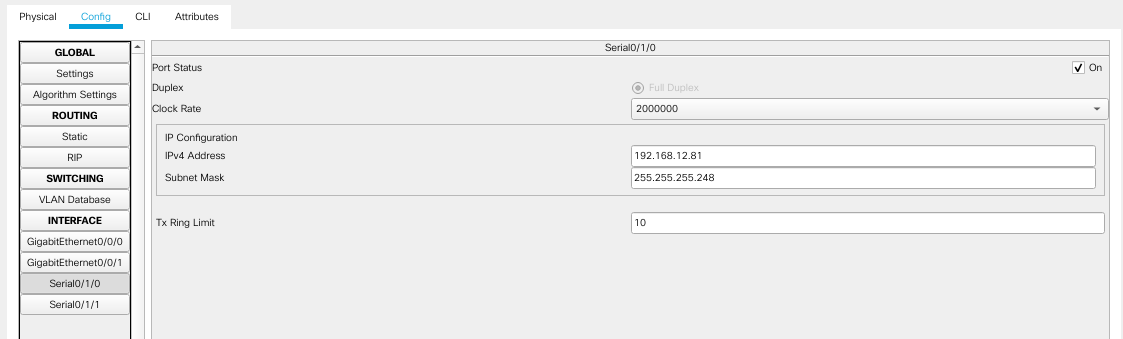
\includegraphics[scale=0.4]{img/9.png}
	\end{center}
	\caption{Настройка первого маршрутизатора}
	\label{fig:9}
\end{figure}

\begin{figure}[H]
	\begin{center}
		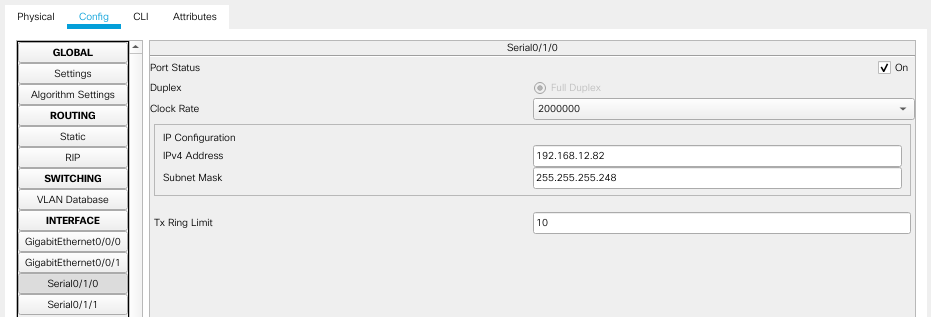
\includegraphics[scale=0.48]{img/10.png}
	\end{center}
	\caption{Настройка второго маршрутизатора}
	\label{fig:10}
\end{figure}

\subsection*{Настройка DHCP сервера для 4-ой подсети}

\begin{figure}[H]
	\begin{center}
		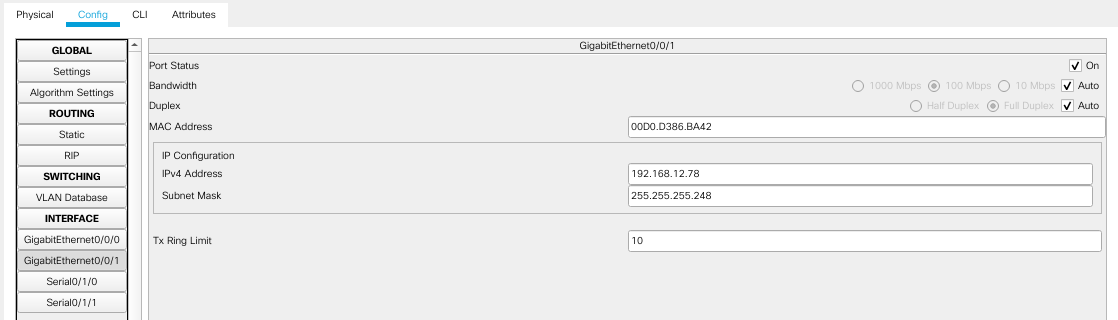
\includegraphics[scale=0.4]{img/11.png}
	\end{center}
	\caption{Настройка муршрутизатора в роли DHCP сервера для подсети №4}
	\label{fig:11}
\end{figure}

\begin{figure}[H]
	\begin{center}
		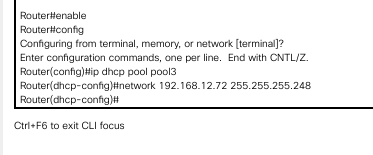
\includegraphics[scale=0.8]{img/12.png}
	\end{center}
	\caption{Настройка маршрутизатора}
	\label{fig:12}
\end{figure}

IP-адреса конечным узлам в подсети выдаются автоматически из диапазона подсети №4 (рис. 13)

\begin{figure}[H]
	\begin{center}
		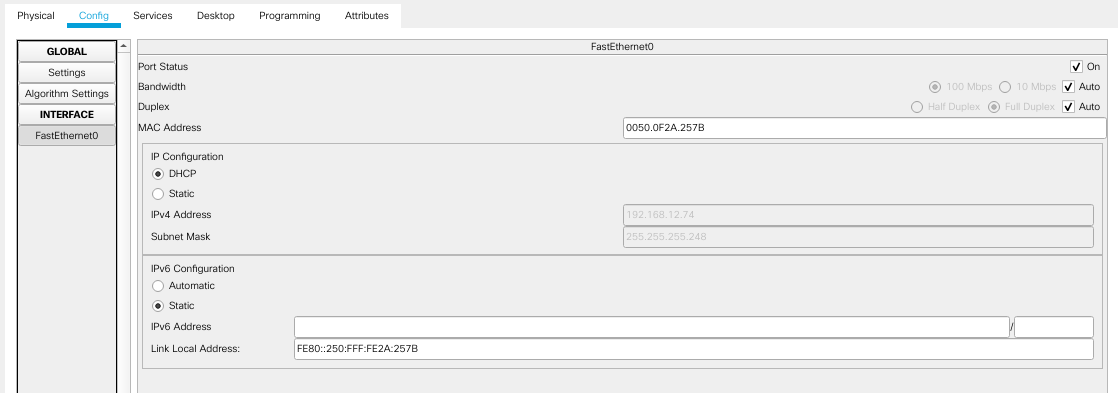
\includegraphics[scale=0.4]{img/13.png}
	\end{center}
	\caption{Автоматически выданный IP-адрес в подсети №4}
	\label{fig:13}
\end{figure}

\subsection*{Настройка DHCP-сервера для 5-ой подсети}

\begin{figure}[H]
	\begin{center}
		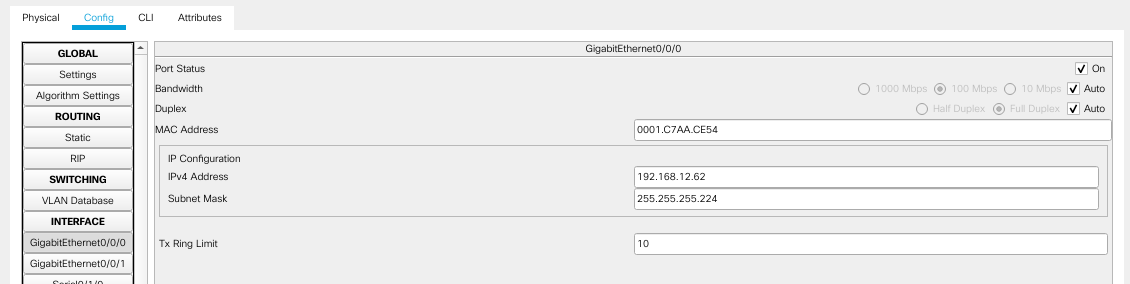
\includegraphics[scale=0.4]{img/14.png}
	\end{center}
	\caption{Настройка маршрутизатора в роли DHCP сервера для подсети №5}
	\label{fig:14}
\end{figure}

\begin{figure}[H]
	\begin{center}
		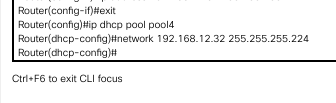
\includegraphics[scale=0.85]{img/15.png}
	\end{center}
	\caption{Настройка маршрутизатора}
	\label{fig:15}
\end{figure}

\begin{figure}[H]
	\begin{center}
		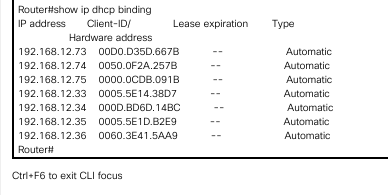
\includegraphics[scale=0.8]{img/16.png}
	\end{center}
	\caption{Результат использование \texttt{show ip dchp binding}}
	\label{fig:16}
\end{figure}

IP-адреса конечным узлам в подсети выдаются автоматически из диапазона подсети №5 (рис. 17)

\begin{figure}[H]
	\begin{center}
		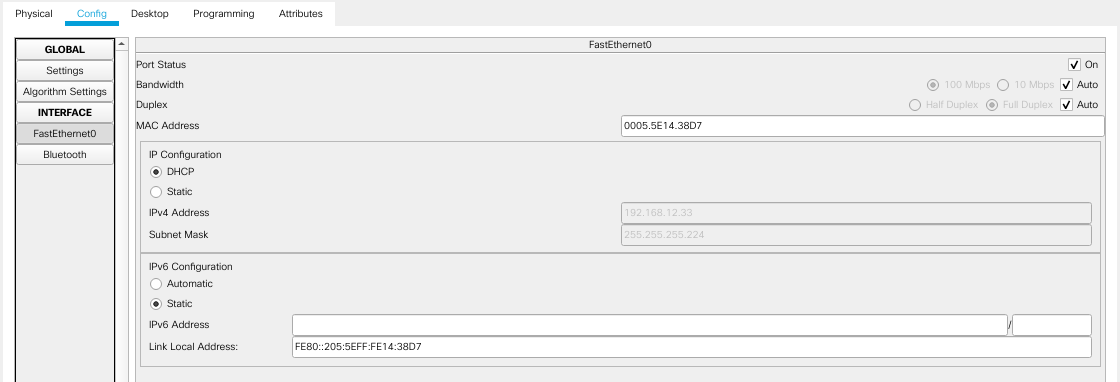
\includegraphics[scale=0.4]{img/17.png}
	\end{center}
	\caption{Автоматически выданный IP-адрес в подсети №5}
	\label{fig:17}
\end{figure}

\subsection*{Проверка с помощью \texttt{ping}}

На риснуке 18 представлены примеры работы команды \texttt{ping}. В первый раз происходит подключение в рамках одной подсети, а во второй происходит попытка подключения к адресу из другой подсети. 

\begin{figure}[H]
	\begin{center}
		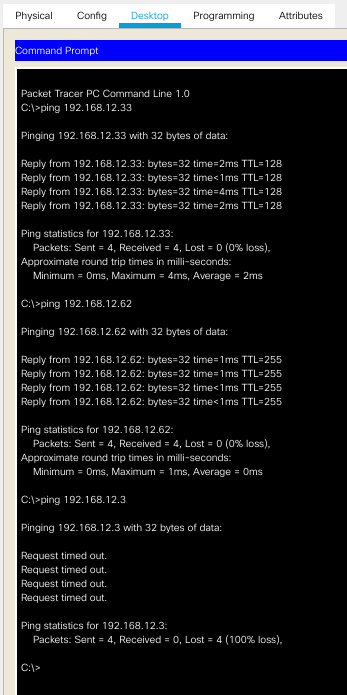
\includegraphics[scale=0.48]{img/18.png}
	\end{center}
	\caption{Широковещательные домены расположены внутри прямоугольников, домены колизий - внутри кругов}
	\label{fig:18}
\end{figure}

\bibliographystyle{utf8gost705u}
\bibliography{51-biblio}
	
\end{document}
